\documentclass[10pt,letterpaper]{article}
\usepackage[margin=0.72in,headheight=12pt]{geometry}
\usepackage[T1]{fontenc}
\usepackage{lmodern}
\usepackage{microtype}
\usepackage{amsmath}
\usepackage{booktabs}
\usepackage{enumitem}
\usepackage{graphicx}
\usepackage{tikz}
\usetikzlibrary{arrows.meta,positioning,fit,calc,backgrounds}
\usepackage{hyperref}
\hypersetup{colorlinks=true,urlcolor=blue!45!black,linkcolor=blue!45!black}
\usepackage{titlesec}
\newcommand{\new}[1]{#1}
\setlength{\intextsep}{6pt}
\setlength{\abovecaptionskip}{4pt}
\definecolor{navy}{RGB}{27,54,82}
\definecolor{pale}{RGB}{237,244,249}
\definecolor{greenpale}{RGB}{237,247,242}
\definecolor{orangepale}{RGB}{253,245,235}
\titleformat{\section}{\bfseries\color{navy}\normalsize}{}{0pt}{}
\titlespacing*{\section}{0pt}{8pt}{3pt}
\setlength{\parindent}{0pt}
\setlength{\parskip}{3.4pt}
\setlist[itemize]{leftmargin=1.35em,topsep=2pt,itemsep=1pt,parsep=0pt}
\pagestyle{empty}

\begin{document}
\begin{center}
{\small\color{navy}\bfseries EEL 5764 \textbar\ Computer Architecture \textbar\ Fall 2026}\par
\vspace{4pt}
{\LARGE\bfseries Output-Column Reuse in a Coherent GEMM Accelerator}\par
\vspace{2pt}
{\large A Controlled Study of Offload Latency and Modeled Hardware Cost}\par
\vspace{5pt}
{\small Yasir Mahmud \quad\textbar\quad Rasin Mohammed Ihtemam
\quad\textbar\quad Mohyeu Hussain}
\end{center}
\vspace{-5pt}
\section{Problem and Research Question}
Matrix multiplication (GEMM) is a useful case for studying the boundary between an out-of-order CPU and a coherent accelerator. A straightforward accelerator kernel computes one output column at a time. For a fixed output row, the same element of matrix $A$ is needed for several neighboring columns, but the one-column loop structure does not explicitly share that value among their accumulators. Computing multiple output columns together exposes reuse and independent arithmetic; it can also require more simultaneous operations and storage. Coherent cache behavior and host invocation overhead may limit the benefit seen by the application.

\new{\textbf{Baseline bottleneck.} In the one-column baseline, every multiply-accumulate loads both \mbox{$A_{ik}$} and \mbox{$B_{kj}$} through the accelerator's coherent cache, so the kernel issues \mbox{$2N^3$} loads and refetches each element of \mbox{$A$} for every output column. These requests share a bounded interface (32-entry queue, at most 4 requests per cycle), and each output's \mbox{$k$}-loop is one serial accumulation chain. We therefore expect the baseline to be limited by coherent-cache request throughput and serialized accumulation, not by arithmetic units.}

\textbf{Research question.} For a fixed-trace, single-invocation GEMM workload, how does the number of output columns computed together affect accelerator offload latency, and what modeled resource cost accompanies the change? We will examine the conditions under which a shorter accelerator schedule translates into a shorter CPU-observed offload interval. We do not assume that more tiling always helps.

\begin{figure}[h!]
\centering
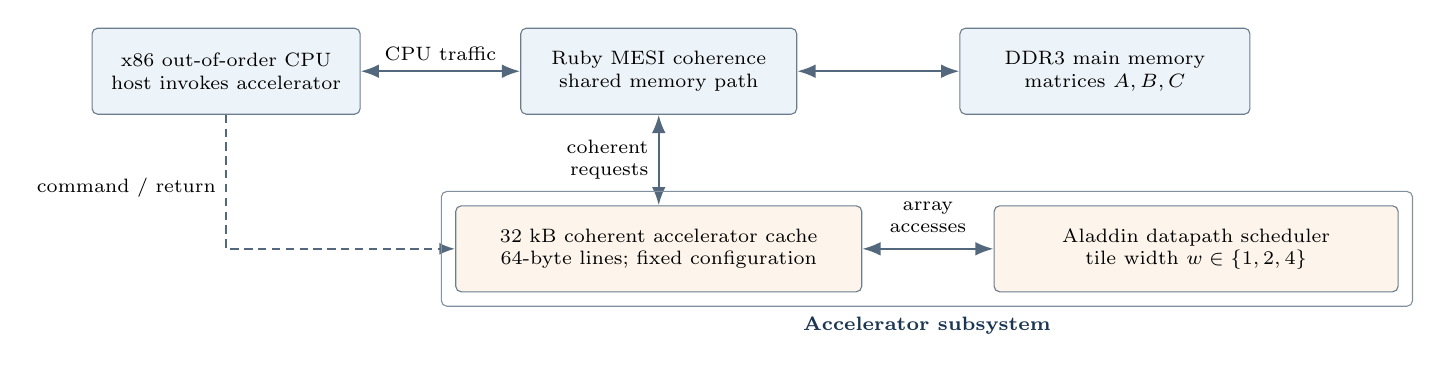
\begin{tikzpicture}[>=Latex, x=0.97in,y=0.8in,font=\scriptsize,
  box/.style={draw=navy!65,rounded corners=2pt,align=center,minimum height=0.43in,fill=pale},
  data/.style={draw=navy!55,rounded corners=2pt,align=center,minimum height=0.34in,fill=greenpale},
  arr/.style={-{Latex[length=2mm]},thick,draw=navy!75}]
  \node[box,minimum width=1.34in] (cpu) at (0,1.05) {x86 out-of-order CPU\\host invokes accelerator};
  \node[box,minimum width=1.38in] (ruby) at (2.23,1.05) {Ruby MESI coherence\\shared memory path};
  \node[box,minimum width=1.45in] (dram) at (4.53,1.05) {DDR3 main memory\\matrices $A,B,C$};
  \node[box,minimum width=2.03in,fill=orangepale] (cache) at (2.23,-0.06) {32 kB coherent accelerator cache\\64-byte lines; fixed configuration};
  \node[box,minimum width=2.02in,fill=orangepale] (dp) at (5.0,-0.06) {Aladdin datapath scheduler\\tile width $w\in\{1,2,4\}$};
  \draw[arr,<->] (cpu) -- node[above]{CPU traffic} (ruby);
  \draw[arr,<->] (ruby) -- (dram);
  \draw[arr,<->] (ruby) -- node[left,align=right]{coherent\\requests} (cache);
  \draw[arr,<->] (cache) -- node[midway,above=2pt,align=center]{array\\accesses} (dp);
  \draw[arr,densely dashed] (cpu.south) |- node[pos=.27,left]{command / return} (cache.west);
  \node[draw=navy!55,rounded corners=2pt,inner sep=5pt,fit=(cache)(dp),label={[font=\scriptsize\bfseries,text=navy]below:Accelerator subsystem}] {};
\end{tikzpicture}
\caption{Architecture used for each comparison. Only the GEMM datapath's output-column tile width changes. The coherence path is modeled; this study does not claim general correctness for arbitrary runtime input changes.}
\vspace{-4pt}
\end{figure}

\section{Mechanism and Expected Tradeoff}
The baseline computes $C_{ij}=\sum_k A_{ik}B_{kj}$ one output at a time ($w=1$). The variants update two or four adjacent sums per inner-loop iteration ($w=2,4$), using one loaded $A_{ik}$ value across those sums (Fig.~2). \new{This targets both baseline limits: \mbox{$A$} loads in the datapath graph fall from \mbox{$N^3$} to \mbox{$N^3/w$}, and \mbox{$w$} independent accumulator chains can proceed in parallel.} The same integer inputs, arithmetic result, host invocation, CPU model, coherence protocol, cache, clock, and simulator patch will be used within each comparison. This is a dataflow transformation represented by Aladdin's generated execution graph, rather than a claim of a new physical chip implementation.

Our hypothesis is that wider tiles can amortize loop and input-use overhead and expose parallel arithmetic, while increasing live accumulators and potentially modeled functional-unit demand. The improvement may plateau when memory service or invocation overhead dominates. We will test these possibilities instead of assuming either outcome.

\begin{figure}[h!]
\centering
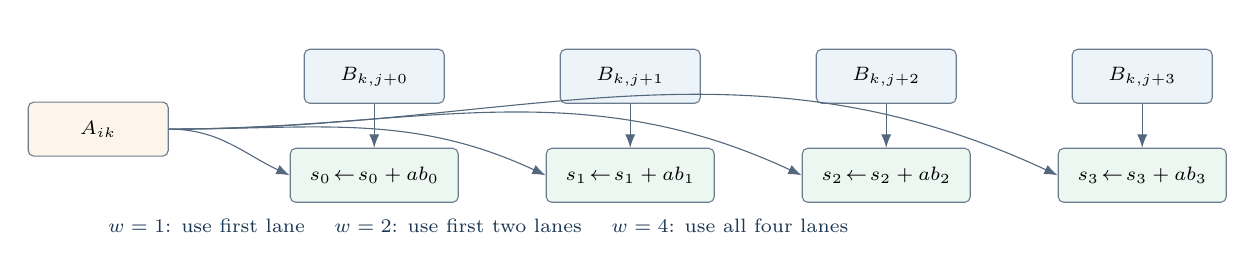
\begin{tikzpicture}[>=Latex,x=1in,y=0.55in,font=\scriptsize,
  node/.style={draw=navy!65,rounded corners=2pt,minimum width=0.70in,minimum height=0.27in,align=center,fill=pale},
  sum/.style={draw=navy!65,rounded corners=2pt,minimum width=0.84in,minimum height=0.27in,align=center,fill=greenpale},
  line/.style={-{Latex[length=1.7mm]},draw=navy!75}]
  \node[node,fill=orangepale] (a) at (0,0) {$A_{ik}$};
  \foreach \j/\x in {0/1.38,1/2.66,2/3.94,3/5.22} {
    \node[node] (b\j) at (\x,0.48) {$B_{k,j+\j}$};
    \node[sum] (s\j) at (\x,-0.42) {$s_{\j}\!\leftarrow\!s_{\j}+a b_{\j}$};
    \draw[line] (b\j) -- (s\j);
    \draw[line] (a.east) to[out=0,in=155] (s\j.west);
  }
  \node[anchor=west,text=navy] at (0,-0.88) {$w=1$: use first lane \quad $w=2$: use first two lanes \quad $w=4$: use all four lanes};
\end{tikzpicture}
\caption{Conceptual output-column tiling: one $A$ value feeds up to four independent accumulators.}
\vspace{-4pt}
\end{figure}

\section{Experimental Methodology}
We will use pinned open-source gem5-Aladdin and Aladdin revisions. \new{We use gem5-Aladdin rather than stock gem5, which cannot model a fixed-function accelerator datapath; it couples Aladdin's pre-RTL timing, power, and area models to gem5's CPU and Ruby memory, so accelerator time and host-observed offload latency are simulated together.}

\new{\textbf{Baseline configuration.} Host: one x86 \texttt{DerivO3CPU} (8-wide, 192-entry ROB, 32-entry load/store queues); Ruby MESI two-level caches with private 64 kB L1D and 32 kB L1I, a shared 2 MB L2, and 1 GB DDR3-1600. Accelerator: Aladdin \texttt{HybridDatapath} with a 32 kB 4-way coherent cache (64-byte lines, 32-entry queue, 4 requests per cycle). All clocks are 1 GHz.} The fixed-trace method records the kernel graph and simulates one accelerator call. A common queue/retry patch and identical configurations apply to all variants. Scripts and effective configurations will be retained so that the comparisons can be reproduced.

\textbf{Study design.} \new{The workload is integer GEMM with deterministic inputs. At \mbox{$N=32$} the three matrices occupy 12 kB, so all sizes fit in the accelerator cache, separating request and dataflow effects from capacity misses; the \mbox{$N^3$} trace graph bounds the largest feasible size.} At both $N=24$ and $N=32$, we will compare $w=1,2,4$. These sizes and widths form a bounded study that separates a width comparison at fixed size from a size comparison at fixed width. Within each pair, only the kernel's tile width changes. \new{A secondary sweep at \mbox{$N=8$} and \mbox{$N=16$} (\mbox{$w=1$} versus \mbox{$w=4$}) will test where the benefit vanishes, with the same kernel on the OoO CPU as a reference.} We will run full element-by-element output checks against a CPU reference, then use a lighter check for timing runs so validation work does not dominate the measured interval. We will retain raw logs and the simulator's effective configuration for each point.

\new{\textbf{Repeated invocation and repeatability.} We will also invoke the accelerator repeatedly with the CPU modifying \mbox{$A$} between calls, check every output after each call, and report the cold first call apart from warm later calls, since the private cache is not flushed. Area estimates will be repeated across independent rebuilds. Stretch goals: \mbox{$w=8$} and a representative inference layer.}

\begin{figure}[h!]
\centering
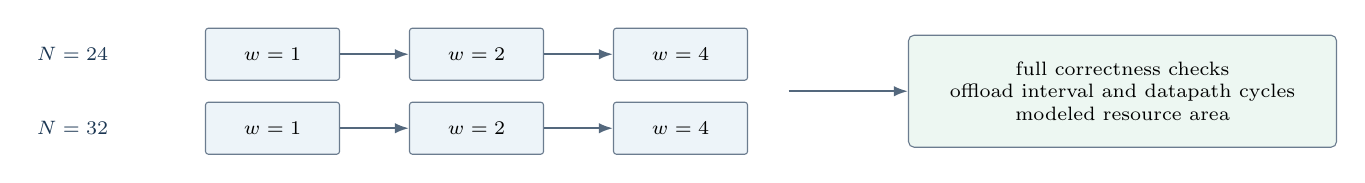
\begin{tikzpicture}[>=Latex,x=1in,y=0.5in,font=\scriptsize,
  cell/.style={draw=navy!65,rounded corners=1pt,minimum width=0.67in,minimum height=0.26in,align=center,fill=pale},
  label/.style={font=\scriptsize\bfseries,text=navy},
  link/.style={-{Latex[length=1.8mm]},thick,draw=navy!75}]
  \node[label] at (0,0.37) {$N=24$};
  \node[label] at (0,-0.37) {$N=32$};
  \node[cell] (a1) at (1.00,0.37) {$w=1$};
  \node[cell] (a2) at (2.02,0.37) {$w=2$};
  \node[cell] (a4) at (3.04,0.37) {$w=4$};
  \node[cell] (b1) at (1.00,-0.37) {$w=1$};
  \node[cell] (b2) at (2.02,-0.37) {$w=2$};
  \node[cell] (b4) at (3.04,-0.37) {$w=4$};
  \draw[link] (a1) -- (a2);
  \draw[link] (a2) -- (a4);
  \draw[link] (b1) -- (b2);
  \draw[link] (b2) -- (b4);
  \node[draw=navy!65,rounded corners=2pt,fill=greenpale,align=center,minimum width=2.14in,minimum height=0.56in] (metrics) at (5.25,0) {full correctness checks\\offload interval and datapath cycles\\modeled resource area};
  \draw[link] (3.58,0) -- (metrics.west);
\end{tikzpicture}
\caption{Study matrix and measurements for each tile-width comparison.}
\vspace{-5pt}
\end{figure}

\section{Metrics and Analysis}
The \textbf{primary metric} is the CPU-observed accelerator offload interval: reset simulator statistics immediately before invocation and end the interval when the blocked host returns. We will also report Aladdin datapath cycles, full-program simulated ticks as a secondary metric, and the tool's modeled functional-unit, memory, and total area estimates. \new{Aladdin's average functional-unit and memory power times datapath cycles gives energy per invocation and, with the offload interval, an energy-delay product; since Aladdin uses a 10 ns power characterization at our 1 ns cycle, these will be compared across widths, not reported as absolute values.} For each fixed $N$, we will report the relative change from $w=1$ and plot offload latency against tile width and modeled area. The whole-program measure will show whether any local accelerator benefit remains visible after setup and host work.

To explain the outcome, we will inspect available datapath and coherent-cache counters, including request counts and access latency, alongside graph size and resource reports. We will distinguish an observed counter change from a proposed cause. If the counters cannot isolate a bottleneck, the report will state that limit. Repeated paired runs will be used where practical to check stability; this deterministic microbenchmark is not intended to support statistical claims about all GEMM workloads.

\textbf{Interpretation rule.} We will treat a datapath-cycle reduction as an internal outcome and judge offload latency separately. We will compare each width's latency with its modeled area rather than declare a universal winner from one metric. If a wider tile helps only at one size, or its cost outweighs its latency benefit, that result will be included and explained.

\section{Deliverables}
The deliverables are the baseline and tiled kernels, scripts/configurations, correctness records, a compact comparison table, plots with labeled units, and a final paper explaining both gains and tradeoffs.

\vfill
{\footnotesize\color{navy}\textbf{Tool provenance:} Harvard ACC \href{https://github.com/harvard-acc/gem5-aladdin}{gem5-Aladdin} and \href{https://github.com/harvard-acc/ALADDIN}{Aladdin}; exact commits, patch, benchmark code, and run scripts are pinned in the project repository.}
\end{document}
